\section{Period Estimation}
We assume that the period of breathing doesn't change abruptly and stay almost constant for each recording. In order to estimate the period we look at the autocorrelation function. For a periodic wave, the autocorrelation function is also periodic with the same period and there are peaks at the integer products of period. So, the period can be estimated by calculating the distances between the peaks. However, since the signal is noisy there are many local maxima, so instead of estimating the distance between peaks, we looked at the autocorrelation function of autocorrelation function of the signal that is being analyzed, and use the location of the maximum of local peaks in the part that is determined by minimum and maximum period. The equation for estimated period is given in \eqref{period_estimation}
\begin{equation}
T' = period_{min} + argmax(R_{R_{x}}[period_{min}:period_{max}])
\label{period_estimation}
\end{equation}
\begin{figure}
	\begin{center}
		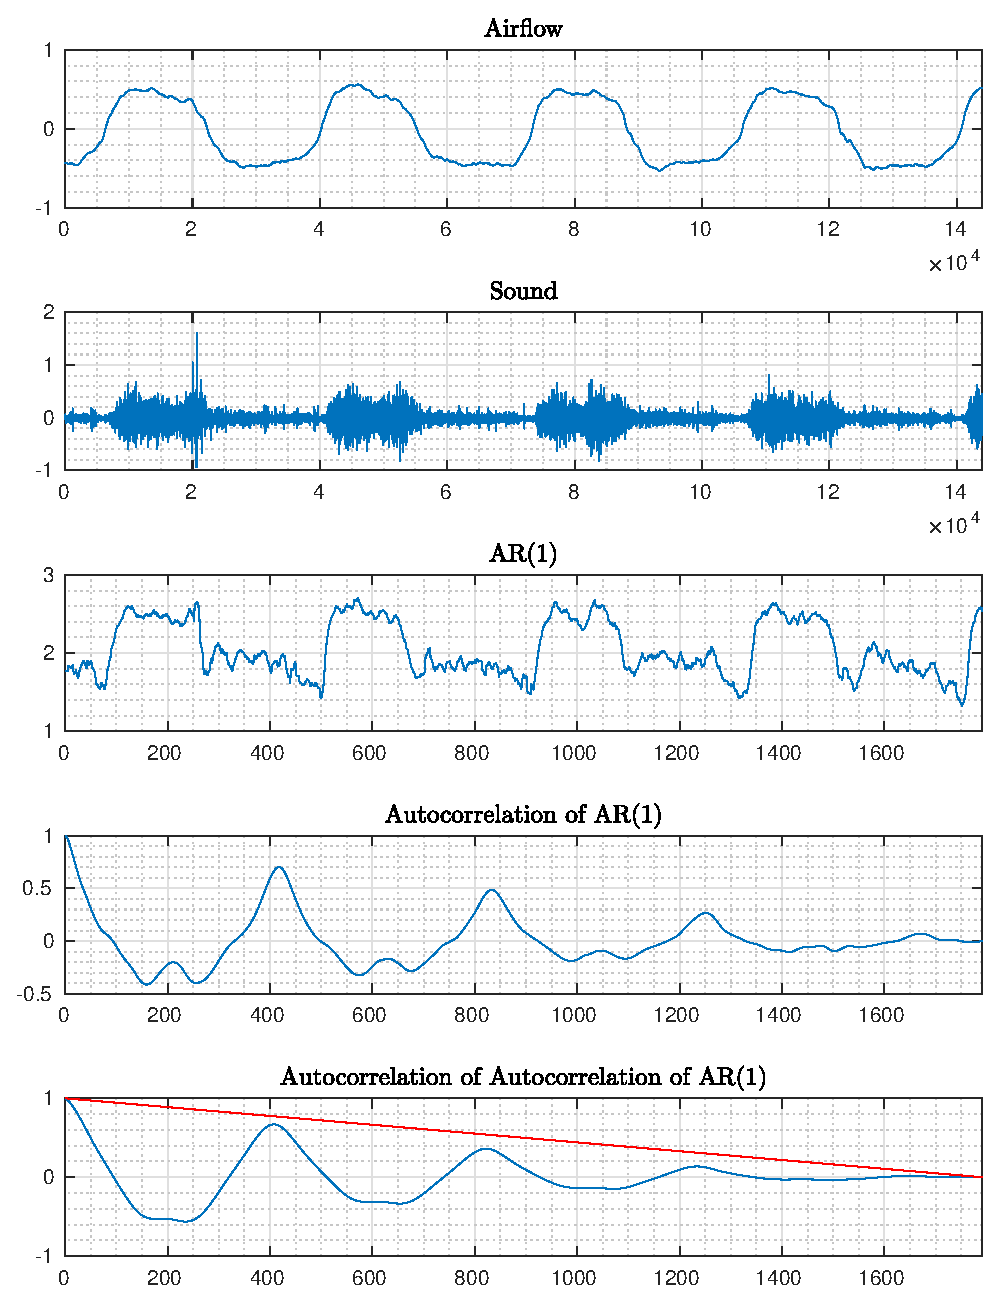
\includegraphics[width=\textwidth]{figures/find_period_ins_exp.eps}
		\caption{Visual Description Of Period Estimation}
		\label{fig:estimate_period}
	\end{center}
\end{figure}
